% 文档类
\documentclass[13pt]{ctexart}
\usepackage{amsmath}
\usepackage{amssymb}
% 设置页面
\usepackage{geometry}
% 插图片
\usepackage{graphicx}
% 设置标题 重命名为英文
\renewcommand{\figurename}{Figure}
\renewcommand{\tablename}{Table}
\renewcommand{\contentsname}{Contents}
% 设置摘要页缩减 
\usepackage{changepage}
% 便于修改字体
\usepackage{fontspec}
% 设置页眉页脚
\usepackage{fancyhdr}
% 清空页眉页脚
\pagestyle{fancy}
% 设置列表缩进
\usepackage[shortlabels]{enumitem}
% 设置修改默认的section标题大小
\usepackage{titlesec}
\titleformat*{\section}{\LARGE}
\titleformat*{\subsection}{\Large}
\titleformat*{\subsubsection}{\Large}
% 使用数学宏包
\usepackage{amsmath}
% 设置表格的列格式
\usepackage{array}
% 三线表宏包
\usepackage{booktabs}
% 设置产考文献不输出默认名
\usepackage{etoolbox}
\patchcmd{\thebibliography}{\section*{\refname}}{}{}{}
% 引入网站作为参考文献
\usepackage{url}
% 设置等宽的代码字体
\setmonofont{IBM Plex Mono}
% 建议这个,但我系统没这个字体,且懒得折腾了 windows用户请
% \setmonofont{Courier New}
% 颜色
\usepackage{xcolor}
% 代码高亮方案宏包
\usepackage{listings}
\definecolor{CPPLight}  {HTML} {686868}
\definecolor{CPPSteel}  {HTML} {888888}
\definecolor{CPPDark}   {HTML} {262626}
\definecolor{CPPBlue}   {HTML} {4172A3}
\definecolor{CPPGreen}  {HTML} {487818}
\definecolor{CPPBrown}  {HTML} {A07040}
\definecolor{CPPRed}    {HTML} {AD4D3A}
\definecolor{CPPViolet} {HTML} {7040A0}
\definecolor{CPPGray}  {HTML} {B8B8B8}
\lstset{
	basicstyle=\ttfamily,
	breaklines=true,
	framextopmargin=50pt,
	frame=bottomline,
	columns=fixed,       
    %numbers=left,                                       % 在左侧显示行号
	frame=none,                                          % 不显示背景边框
	backgroundcolor=\color[RGB]{255,255,255},            % 设定背景颜色
	keywordstyle=\color[RGB]{40,40,255},                 % 设定关键字颜色
	numberstyle=\footnotesize\color{darkgray},           % 设定行号格式
	commentstyle=\itshape\color[RGB]{0,96,96},                % 设置代码注释的格式
	stringstyle=\slshape\color[RGB]{128,0,0},   % 设置字符串格式
	showstringspaces=false,                              % 不显示字符串中的空格
	language=python,                                     % 设置语言
	morekeywords={alignas,continute,friend,register,true,alignof,decltype,goto,
		reinterpret_cast,try,asm,defult,if,return,typedef,auto,delete,inline,short,
		typeid,bool,do,int,signed,typename,break,double,long,sizeof,union,case,
		dynamic_cast,mutable,static,unsigned,catch,else,namespace,static_assert,using,
		char,enum,new,static_cast,virtual,char16_t,char32_t,explict,noexcept,struct,
		void,export,nullptr,switch,volatile,class,extern,operator,template,wchar_t,
		const,false,private,this,while,constexpr,float,protected,thread_local,
		const_cast,for,public,throw,std},
	emph={map,set,multimap,multiset,unordered_map,unordered_set,numpy,graph,path,append,extend,
		unordered_multiset,unordered_multimap,vector,string,list,deque,
		array,stack,forwared_list,iostream,memory,shared_ptr,unique_ptr,
		random,bitset,ostream,istream,cout,cin,endl,move,default_random_engine,
		uniform_int_distribution,iterator,algorithm,functional,bing,numeric,},
	emphstyle=\color{CPPViolet}, 
}

\begin{document}
\newgeometry{top = 1cm, right = 2.54cm, left = 2.54cm, bottom = 2.54cm}
% 第一页的字体为times new roman
\setmainfont{Times New Roman}
\thispagestyle{empty}

\begin{table}[h]
    \quad { }  \begin{minipage}[t]{5.5cm}
        % arraystretch 是调节列高
        \begin{tabular}[t]{>{\centering\arraybackslash}b{10em}}
            \fontsize{12pt}{10pt}\selectfont \textbf{Problem Chosen}\\ [2pt]
            {\color{red} \fontsize{20pt}{10pt}\selectfont B}
        \end{tabular}
    \end{minipage}
    \begin{minipage}[t]{5.2cm}
        \begin{tabular}[t]{>{\centering\arraybackslash}p{10em}}
            \fontsize{12pt}{10pt}\selectfont \textbf{2021} \\ [-2pt]
            \fontsize{12pt}{10pt}\selectfont \textbf{MCM/ICM} \\ [-2pt]
            \fontsize{12pt}{10pt}\selectfont \textbf{Summary Sheet}
        \end{tabular}
    \end{minipage}
    \begin{minipage}[t]{3cm}
        \begin{tabular}[t]{>{\centering\arraybackslash}b{12em}}
            \fontsize{12pt}{10pt}\selectfont \textbf{Team Control Number} \\ [2pt]
            {\color{red} \fontsize{21pt}{10pt}\selectfont 2106317}
        \end{tabular}
    \end{minipage}
\end{table}
\vspace{-20pt}
\noindent{\rule{\textwidth}{0.5mm}}

% 标题
{\centering\fontsize{18}{16}\selectfont\textbf{{Trajectory Planning of Drone Formation Based On Artificial Fish Swarms Algorithm}}
% 摘要
\vspace{10pt} 

\fontsize{13}{10}\selectfont\textbf{{Summary}}\par}

\vspace{10pt}

% 正文字体 13 pt
\fontsize{13}{12.5}\selectfont

\begin{adjustwidth}{1cm}{1cm}
\indent { }{ }{ }{ }{ }{ }Australia has seen big wildfires in recent years. When fighting a fire, the SSA drones used by the fire brigade for communication and fire observation is the shining star in the fight against the fire. However, in the face of the two antagonistic demands of economy and safety, it is of great significance to use SSA drones with the least budget to ensure the safety of firefighters.
In order to get the optimal number of drones, we established a drone flight planning model based on artificial fish school algorithm. By generating environmental variables in a specific disaster relief area, and then optimally planning the orbits of different numbers of SSA drones, we get the cost and safety performance of arranging a specific number of drones. Through our simulation experiment in a forest-urban area in Victoria, we have obtained that a single EOC fire brigade that safely controls a 5x5 km requires 15 SSA drones and 4 radio repeaters drones.

In the model, we quantitatively describe the possibility and hazard of fire at a specific location based on fire data over the years. Each SSA drone executes a predetermined drone trajectory cooperation scheme to make the trajectory close to the optimal. Therefore, by calculating the safety performance of different tracks, we have obtained a scheme that guarantees the safety and uses the least cost to improve the highest performance. All orbital schemes and indicators for evaluating their performance can be quantified and visualized.

In order to study how the model adapts to extreme fire conditions in the next 10 years, we combined with the climate conditions in a specific area and called the gray prediction model to get the wildfire trend in the next decade. We generate predicted environmental data from these trends, and perform another simulation on the existing orbit planning model. We found that the model will perform well in the next 6 years.
Considering the influence of altitude on the radio repeater drone, we then add altitude information to the environmental variables, and optimize the position through the traditional artificial fish swarm algorithm.

Sensitivity analysis shows the strong robustness of our model and the importance of setting constant parameters to the algorithm. Later, we will combine the geographic location and urban distribution of Victoria Forest to write a drone budget table with purchase basis to the Victorian government.


\vspace{10pt}
\textbf{key words} : Artificial fish swarm algorithm; Quantitative visualization; Grey prediction; 
\end{adjustwidth} 

%% 开始写 memo 信
%% 更换字体为 palatino 也可以不换
%\setmainfont{texgyrepagella-regular.otf} 
%\newpage
%\newgeometry{left = 3.5cm, right = 3.5cm}
%\thispagestyle{empty}
%
%{\centering \fontsize{18pt}{14pt}\selectfont \textbf{MEMO}\par}
%
%\noindent FROM: Team {} 1917694 , MCM C
%
%\noindent To: The group of Governors
%
%\noindent Date: January 28, 2019
%
%\vspace{10pt}
%
%Dear Officials:
%
%It is our honor to help you with analyzing the spread and characteristics of opioid. We are writing this letter to report our findings.
%
%We analyzed the characteristics of opioid spread in the five states and counties, and found that if left uncontrolled, the opioid abuse will continue to spread, and the number of drug users will increase. We also found that there is no obvious relationship between the spread of opioid use and the geographical location. We deduced that Ohio is most likely the originated state of opioid use, and the drug cases will increase significantly over time. Of all five states, West Virginia shows a relatively healthy status. We also analyzed each county in the five states. Taking West Virginia as an example, Monongalia and Berkeley may be the originating counties for heroin transmission, and drug cases in these two counties are mainly spread to Kanawha and Berkeley.
%
%We determined two epidemic thresholds based on characteristics of opioid spread, with respect to the number of opioid cases and opioid spread rate respectively. We found that the number of narcotic analgesics cases in Ohio reaches the threshold in 2022, and the number of heroin cases in Pennsylvania reached the threshold in 2023.
%
%We analyzed the correlations between the number of opioid cases and various socio-economic factors. We found that the number of opioids cases shows high correlations with disability status, educational level, family status and adolescents. Therefore, we provide suggestions based on these factors to help suppress opioid spread. We also evaluate the effectiveness of these strategies. The result shows that when the amount of drug spread is less than 26.3\% on before, the number of drug users will be significantly reduced in 3 years, and become lower than that of 2010 in 5 years. 
%
%We also do sensitivity analysis of our model. We found that inflows of drugs from outside the states also plays an important role in affecting the number of opioid cases.
%
%Based on our analysis, we provide some suggestions to effectively prevent opioid spread:
%
%1. National and local governments play an important role in detecting and preventing opioid overdose and abuse. Monitoring systems and early warning mechanisms should be established to effectively detect and respond to the spread of opioid abuse.
%
%2. Provide more job opportunities to alleviate people's pressure, even to set up a free subsidy program. The local government should also publicize the harm of opioids abuse.
%
%3. Prescriptions and sales of opioids should be strictly controlled, and a feedback mechanism for mandatory postoperative hospital visits should be established. The patients should also be examined for abuse of opioids during the hospital examination.
%
%4. Impose careful check and strict management of logistics, to reduce the impact of opioids from outside the states.
%
%We believe that our model is useful for preventing opioid spread in the future. You are welcome to contact us at any time for further cooperation.
%
%% 信多出一页,清理页眉页脚
%\thispagestyle{empty}
%% 信的结尾
%{\raggedleft
%Sincerely yours
%
%MCM C Team 1917694\par
%}

% 目录页
\newpage
\thispagestyle{empty}
\tableofcontents
\newpage
% 目录页后面是第一页
\setcounter{page}{1}

% 开始写正文
% 设置正文的页边距
\newgeometry{top=3cm, left=3.5cm, right=3.5cm}
% 设置正文的页眉页脚
\fancyhf{}
\fancyhead[C]{ }
% 此处修改右上角页码
\fancyhead[R]{Page \thepage\ of 18}
%\fancyhead[R]{Page \thepage\ of 15}
\fancyhead[L]{Team \# 2106317}
\fancyfoot[C]{\bfseries\thepage}
\textbf{\section{Introduction}}
\textbf{\subsection{Background}}
From 2019 to 2020, devastating wildfires occurred in all states of Australia, with the worst impact in New South Wales and eastern Victoria. To monitor the fire, firefighters have used drones for surveillance and situational awareness(SSA). Drones are divided into SSA drones and Radio Repeater drones. It is necessary to design the number of drones  and the combination of drone formations.
\textbf{\subsection{Restatement of the Problem}}
Consider the background information, the requirements identified in the problem statement, and the information provided in the problem attachment to address the following issues.

\begin{itemize}
	\item In order to purchase for a proposed new division, “Rapid Bushfire Response”, of Victoria’s Country Fire Authority (CFA), a model needs to be created to determine the optimal number and combination of SSA drones and Radio Repeater drones. The model needs to consider capability and safety with economics, and consider observational and communications mission needs and topography. In addition, your model should also incorporate fire event size and frequency as parameters.
	\item Explain how your model adapts to the changing likelihood of extreme fire events in the next decade, and if the cost of the drone systems stays constant, how much equipment cost is expected to increase.
	\item Determine a model for optimizing hovering VHF/UHF radio-repeater drones on different terrains with different levels of firepower. An example map is given.
	\item Prepare a one- to two-page annotated Budget Request supported by your models for CFA to submit to the Victoria State Government.
\end{itemize}
\textbf{\subsection{Our Works}}

\begin{itemize}
	\item First, we build a model to analyze the optimal number and combination of drone to purchase, and determine the selection based on the model.
	\item Then we estimate the equipment cost based on the predicted development and transformation in ten years.
	\item We use artificial fish swarms algorithms to plan the drone path of action reasonably, and determine the route by considering fire event size and frequency as parameters. And then optimize the position of VHF/UHF radio-repeater drones in r fires of different sizes on different terrains.
	\item Finally we will write a  one- to two-page annotated Budget Request supported by our models. 
\end{itemize}
\textbf{\section{Assumptions and Notations}}
\vspace*{-10pt}
\textbf{\subsection{Assumptions}}
Due to the lack of necessary data, we make the following assumptions to help us perform modeling.
\begin{itemize}[itemsep=0.3ex, leftmargin=1.2cm]
	\item[1.] Assuming that multiple WileE-15.2X hybrid drones are used in the deployment process, which are equipped with monitoring equipment and repeaters. The drones, monitoring equipment and repeaters are in good working condition, and air resistance and weather are ignored during the flight. Keeping the maximum flight speed of 20m/s moving at a constant speed, the flight height will not affect the flight status of the drones.
	\item[2.]  Assuming that the drone mission environment is a rectangular area mainly composed of the wildfire-prone areas in Victoria in recent years, the environmental model is appropriately simplified, and the map is simplified to a distribution map of flat areas and rugged areas according to the terrain and urban-rural distribution. And according to the wildfire data in recent years, corresponding to the latitude and longitude coordinates, set the corresponding parameters of the coordinates. According to known conditions, the range of the handheld radio carried by the forward personnel is 5km in the flat area and 2km in the urban area. This is equivalent to the SSA drones' monitorable signal range of 5km and 2km in the flat area and the urban area respectively. 
	\item[3.]Assuming that the EOC position is fixed, the drone carrying the repeater will hover after reaching the position, and the radio signal will not be affected by weather factors
\end{itemize}
\textbf{\subsection{Notations}}
Here are all the notations and their meanings in this paper.
\begin{table}[h]
	\centering
	\vspace{3pt}
	\begin{tabular}{>{\centering\arraybackslash}p{5em}>{\centering\arraybackslash}p{30em}}
	\toprule % 绘制第一条线
	Symbol & Meaning \\ \midrule
	$X_i$ & Drone location \\
	Visual & Artificial fish field of view \\ 
	$E_i$ & Longitude of coordinate point \\
	$W_i$ & Latitude of coordinate point\\ 
	$P_{f_i}$ & Probability of fire at coordinate point\\
	$\delta_i$ & Drone charging desire\\
	$L_i$ & Drone track length \\
	$d_i$ & Distance from charging point \\
	$\varepsilon_i$ & Remaining battery $t$ \\
	$J_i$ & Various cost functions \\
	$Y_i$ & Evaluation function \\
	$\eta_{i}$ & Refreshing rate \\
	\bottomrule
	\end{tabular}
\end{table}

\textbf{\section{Optimal Combination of Drones(Question 1)}}

\textbf{\subsection{Environment Modeling}}
We use grid method to divide the planning space. The track is connected by adjacent grid nodes. Each grid node contains the longitude and latitude coordinates, fire probability and terrain information (city or forest) in the planning environment, and records the point Refresh rate.

\begin {figure}[h]
\centering % 居中显示
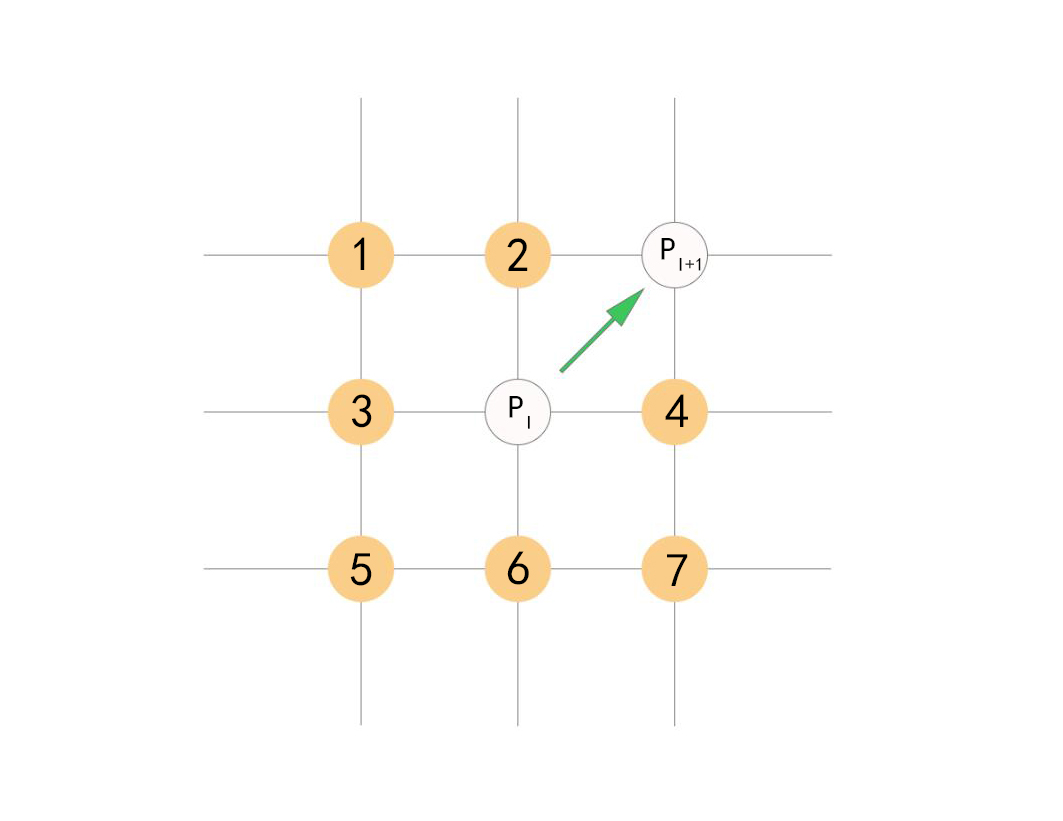
\includegraphics[width=13cm,height=5.5cm]{node.jpg}
\caption{Node diagram} % 标题
\label{node}
\end {figure}

Figure \ref{node} depicts the link of track points, that is, the next node of each node intelligently appears in eight adjacent nodes. Thus, the trajectory planning can be described as:
\begin{equation}
	S(x_s,y_s)\stackrel{\Gamma(q)}{\longrightarrow}P_1(x_1,y_1)…P_{n-1}(x_{(n-1)},y_{(n-1)})
	\stackrel{\Gamma(q)}{\longrightarrow}G(x_g,y_g)
	\label{Node}
\end{equation}
Formula \ref{Node} $S(x_s,y_s)$ is the starting point ; $G(x_g,y_g)$is the target point ; $P_1(x_1,y_1) … \\ P_{n-1}(x_{(n-1)},y_{(n-1)})$ is the intermediate track node; $\Gamma(q)$ represents the constraint condition; $q$ is the track constraint parameter.

More importantly, to refine the environmental conditions, we visualized the fire probability of the map, and selected the rectangular area in the map where the fire probability distribution and the city / forest distribution are more suitable. 

\begin {figure}[htb]
\centering % 居中显示
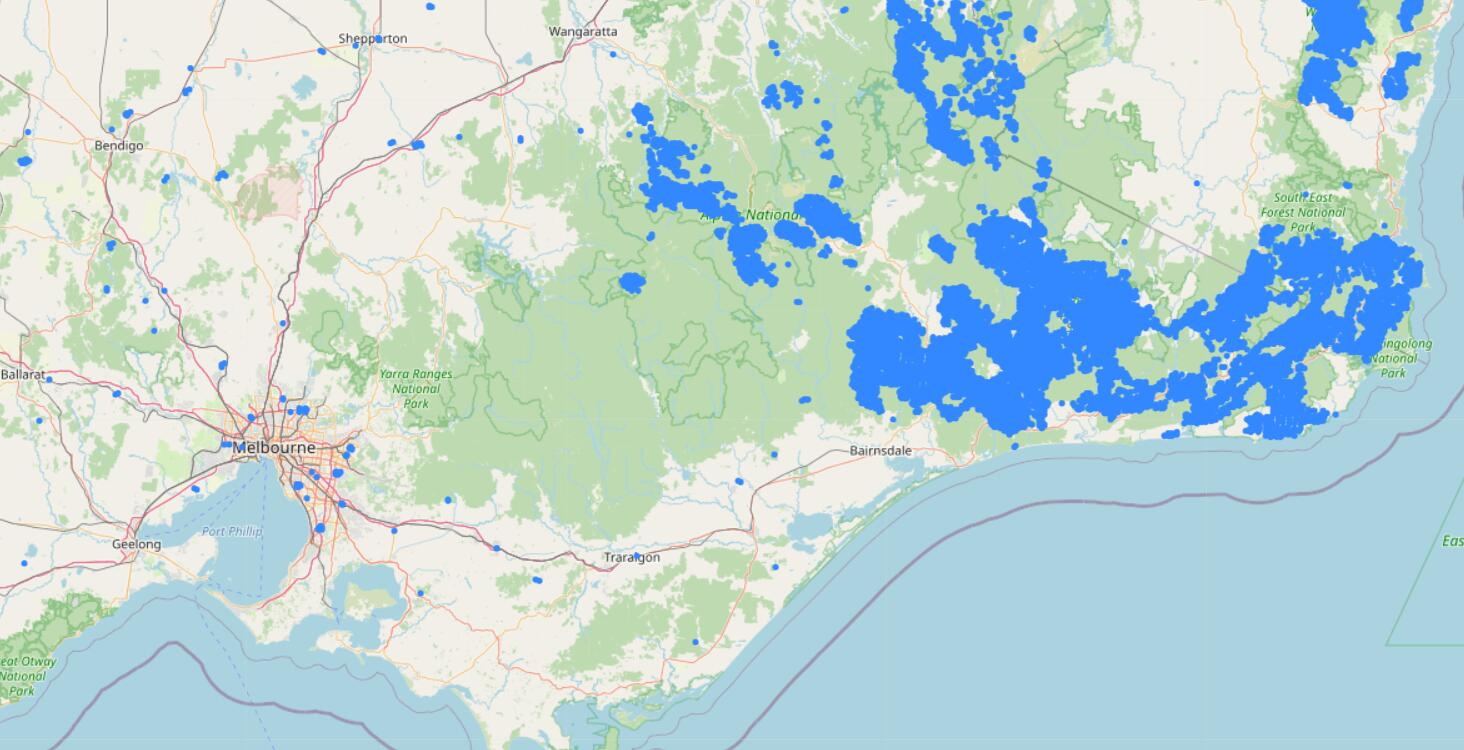
\includegraphics[width=0.9\textwidth]{ff.jpg}
\caption{Wildfire probability distribution map of Victoria} % 标题
\label{ff}
\end {figure}

As is illustrated in Figure \ref{map}, the longitude and latitude coordinates of the four corners of the rectangular region are:
\begin{equation}
	\begin{cases}
	(-37.790163, 148.017149), (-37.790163, 148.567343),& \\
	(-37.413923, 148.017149), (-37.413923, 148.567343) &
	\end{cases}
\end{equation}

\begin {figure}[htb]
\centering % 居中显示
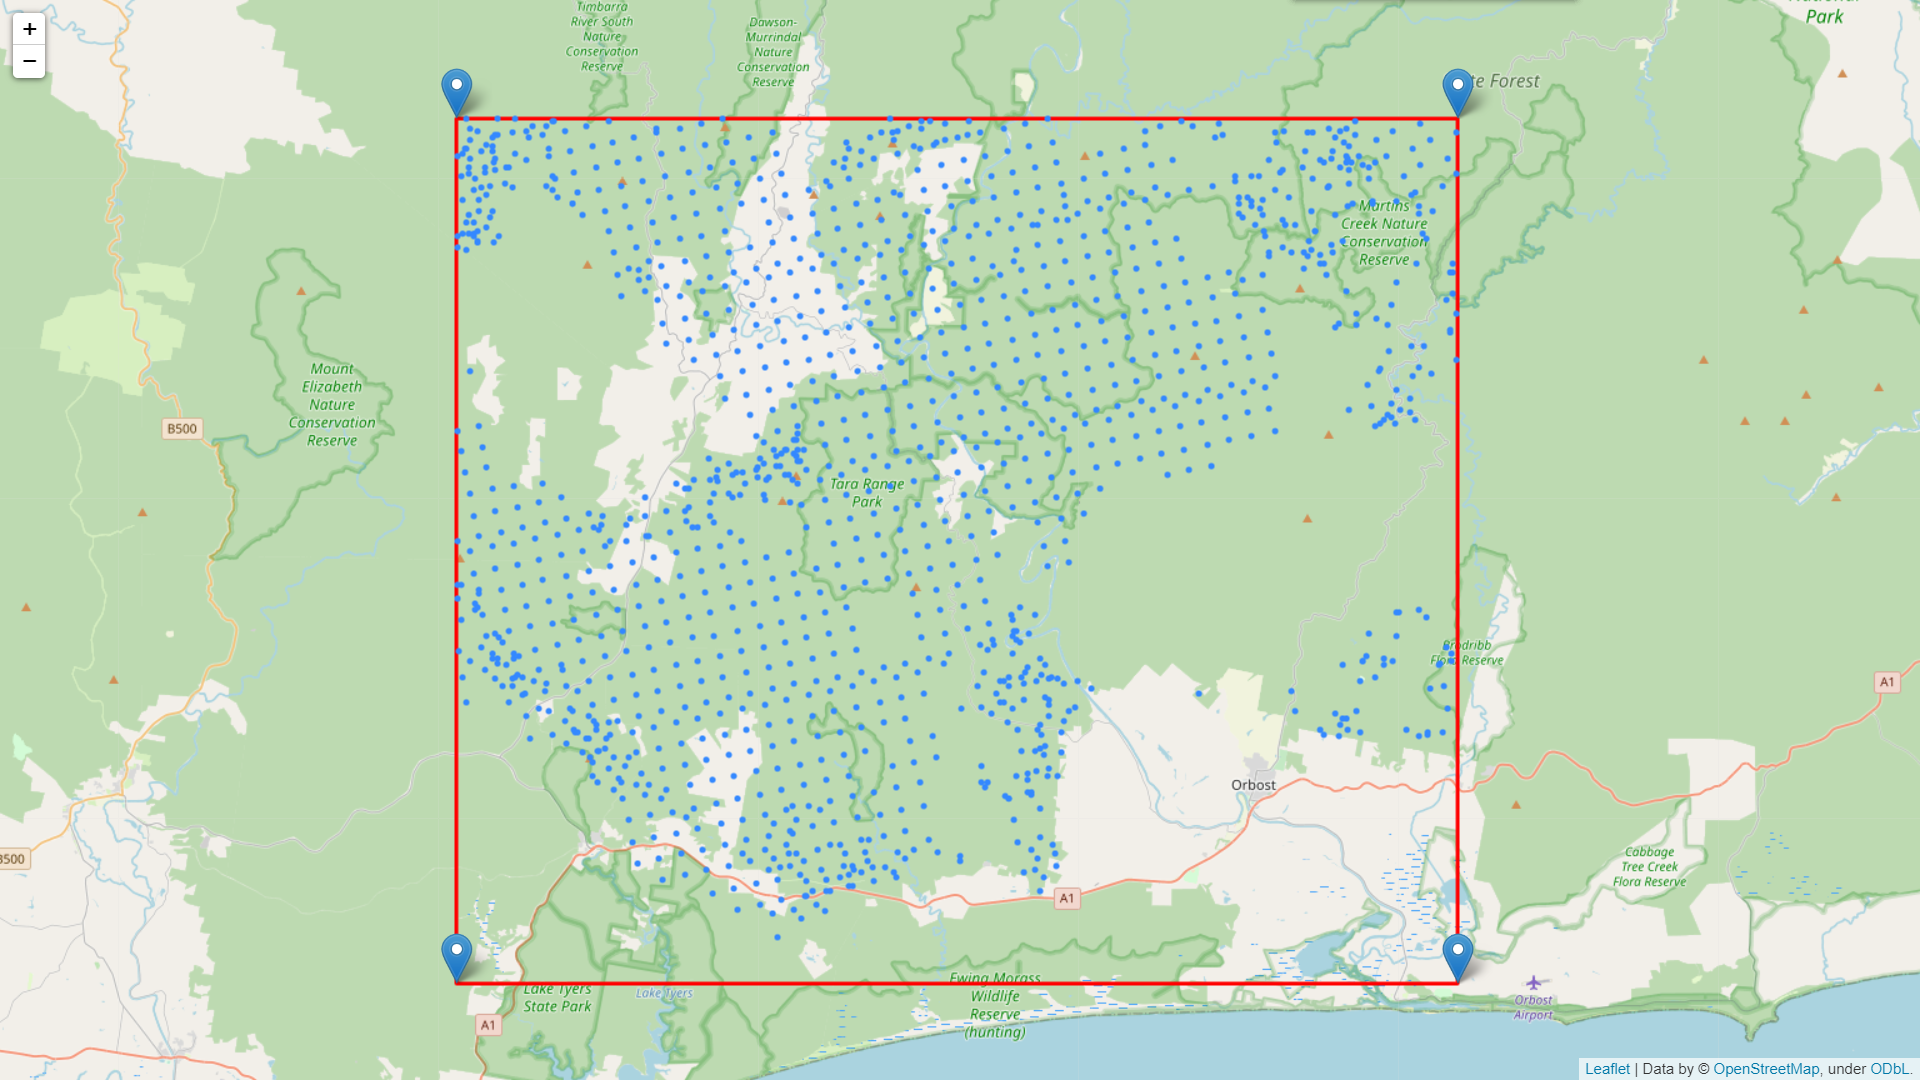
\includegraphics[width=0.9\textwidth]{map.png}
\caption{Target region overview} % 标题
\label{map}
\end {figure}


\textbf{\subsection{Determine Details of Algorithm }}

In the artificial fish school algorithm, the topographic map is abstracted as a two-dimensional plane containing only coordinate points, and each coordinate point records information, including the probability of future fire at that point and the refresh frequency.
At each moment, at least one drone's monitoring signal range can cover the coordinate point, then the coordinate point is said to be safe; if the coordinate point is out of the monitoring signal range of all drones from a certain moment, then from that moment Ts starts to record the time until the coordinate point is covered by the drone monitoring signal again (recorded as Te at this time), this time period is called the refresh time $Tr=Te-Ts$
Define refresh frequency: refresh time divided by unit time
Treat the drone as an artificial fish, set it in the target search space, there are N artificial fish forming a formation,
The vector represents the individual state of the artificial fish, including charge desire
Define the desire to charge: the desire to go to the charging point that determines the charging needs such as the distance from the charging point and the remaining power. This desire is higher than the desire to charge when looking for food.
The current food concentration of the artificial fish is the refresh frequency. The planning goal is to make the refresh frequency of the coordinate points within a specific range reach a higher level, select a specific number of artificial fish, record and compare the refresh frequency and cost of the coordinate points when the target is reached Cost, comprehensive consideration of efficiency and cost, to arrive at the best UAV arrangement strategy


According to the actual situation and budget constraints, set the range of the number of drones to . For each possible number of drones, call the artificial fish school algorithm for planning and testing, and record the number of drones when the target is reached Refresh frequency and cost of time coordinate points, and finally get the best UAV formation number.

\textbf{Define the foraging behavior of artificial fish.}\quad Suppose that the current status of the $i$ artificial fish is$X_{i}=(E_{i},W_{i},P_{f_{i}},\delta_{i})$, charge desire is $\delta_{i}=f(d_{i},\varepsilon_{i})$, the refresh rate function for the current location is $P_{r_{i}}=f(T)$. On the basis of the following equation, check the state of the surrounding eight points within the range of perception  $X_{V}=(X_{1},X_{2},\cdots,X_{8})$ and the refresh rate of each status$P_{f_{i}}=(P_{f_{1},P_{f_{2}},\cdots,P_{f_{8}}})$.
\begin{equation}
	{X_{V}=X+visual \cdot rand()}
	\tag{2.1}
\end{equation}
Then obtain the minimum fire probability state point in the nearby lattice, we establish the following equation and move the fish as follows so that $X_{i}$ could reach a new state:
\begin{equation}
	{X_{next}=X+\frac{X_{v}-X}{\left \|X_{v}-X \right \|} \cdot step \cdot rand()}
	\tag{2.2}
\end{equation}

\textbf{Define the charging behavior of artificial fish.}\quad The distance from the charging point $d_{i}$ and the remaining power $\sigma_{i}=f(L_{i})$ determine the charging desire to the charging point $\varepsilon_{i}=f(d_{i},\sigma_{i})$, when this index is higher than the foraging desire$\phi_{i}=f(P_{f_{i}})$, return to the charging point. Therefore, we establish the following equation:
\begin{equation}
	X_{next} =  \begin{cases}
		X+\frac{X_{v}-X}{\left \|X_{v}-X \right \|} \cdot step \cdot rand(),& \varepsilon_{i}<\phi_{i} \\
		X_{charge},& \varepsilon_{i}\geq\phi_{i}.
	\end{cases}
\end{equation}


\textbf{Define the anti clustering behavior of artificial fish.}\quad Each artificial fish moves to the center far away from its companion as far as possible in the process of swimming, so as to prevent overcrowding and flight direction aggregation. 
Suppose that the current status of the $i$ artificial fish is$X_{i}=(E_{i},W_{i},P_{f_{i}},\delta_{i})$, charge desire is $\delta_{i}=f(d_{i},\varepsilon_{i})$, the refresh rate function for the current location is $P_{r_{i}}=f(T)$. Take the position of the current fish as the center, the number of artificial fish within its sensing is $N_{f}$ and these fish form an aggregate$S_{i}$.The fish aggregate obeys the following formula.
\begin{equation}
	S_{i}={X_{i}|\left \|X_{j}-X_{i}\right \| \leq visual,j=1,2,\cdots,i,i+1,\cdots,n}
	\tag{3}
\end{equation}
If the aggregate $S_{i}\neq\varnothing$ ($\varnothing$ means a empty set), it illustrates that there is at least one artificial fish in the perceptual range of the $i$ artificial fish, namely $N_{f}\geq1$.Then check the status of the points $X_{V}$ in the aggregate$S_{i}$ and the refresh rate $P_{r_{i}}$ of each state, find out the minimum refresh rate state point $minP_{r}$ in the nearby lattice. Thus, we find the center position of the aggregate $X_{center}$ and the fish moves forward towards the position.The trajectory accords with the following equation:
\begin{equation}
	X_{next}=X+\frac{X_{centre}-X}{\left \|X_{centre}-X \right \|} \cdot step \cdot rand()
	\tag{4}
\end{equation}
If the aggregate $S_{i}=\varnothing$($\varnothing$ means a empty set), it indicates that there is no other artificial fish in the perceptive range of artificial fish $i$, namely$N_{f}=0$. Then it will perform foraging behavior.



\textbf{\subsection{Determining the Price Function}}

\textbf{Define the fire threat cost.}\quad We determine the formula below to describe the fire threat cost quantitatively.
\begin{equation}
	J_{F}=\sum_{i=1}^{n}J_{F-i}
\end{equation}
$J_{F-i}$ refers to fire threat cost of UAV in track segment $i$. Its detailed model is as follows:
\begin{equation}
	J_{F-i}=\sum_{i=1}^{n}J_{F-i}=\sum_{i=1}^{n}(\mu P^i_{ff_{j}}+(1-\mu)P^i_{fs_{j}})
\end{equation}
$J_{F_{j}-i}$ refers to the cost of fire threat to the surrounding points in track segment $i$; $N_{F}$ means the sum total of fire threat;$P^i_{ff_{j}}$ and $P^i_{fs_{j}}$ refers to the fire threat index of track segment $i$, namely the frequency and scale of wildfires.

\textbf{Define the refresh interval cost.}\quad We also suppose the cost function of refreshing interval for information stored on coordinate points.
\begin{equation}
	J_{F}=\sum_{i=1}^{n}J_{T_{i}}
\end{equation}
$J_{T_{i}}$ represents refresh interval cost of UAV in track segment $i$. Its detailed model is listed below: 
\begin{equation}
	J_{T_{i}}=\sum_{k}^{S_{m}}\eta_{i_{k}}
\end{equation}

In the above equation, $\eta_{i_{k}}$ refers to the refresh time interval of each point corresponding to the coordinate set in track segment $i$; $S_{m}$ equals to the aggregate of coordinates corresponding to each position in the track segment $i$.


\textbf{\subsection{Determining the Objectives of the Model}}
\textbf{Determining the Minimization Function of Track Model}
In order to realize the optimal formation design, the track model minimization function is established.
\begin{equation}
	J=min\sum_{\tau=1}^{n}(\omega_{1}J^{\tau_{F}}+\omega_{2}^{\tau_{T}})
\end{equation}
In the above formula, $\omega_{k},k=1,2$ refers to the weight of each cost while $J^\tau_{F}$ and $J^\tau_{T}$ represents the cost of fire threat and refreshing time interval for the $i$ drones in the formation.

\textbf{Determining the Evaluation of the Model}
Determine an indicator called \textbf{performance} to evaluate the performance of formations with different number of SSA drones. The performance of each point in the map matrix should at least reach the qualified level. And the fire probability is positively correlated with the refresh rate which means that the point with high fire probability should also have a higher refresh probability. The evaluation function is listed below:
\begin{equation}
	Y_{i}=max\sum_{\i=1}^{n}((\gamma)P_{ff_{i}}+(1-\gamma)P_{fr_{i}}\cdot\eta_{i})
\end{equation}

\textbf{\subsection{Algorithm Flow of Artificial Fish Swarm Planning}}

The first step is to initialize the size of the fish swarm, define the moving step size and searching range, iterative threshold and crowding degree of the artificial fish; the second step is to record the position and food concentration of the artificial fish in the field of vision at random; the third step is to calculate and select the next step of the artificial fish behavior and update it; the fourth step is to select the optimal position of the fish swarm; the fifth step is to judge whether it has reached the pre-set of the algorithm If the termination condition of the stroke design has been reached, the result of the operation will be output; if not, return to step 3.

\begin {figure}[h]
\centering % 居中显示
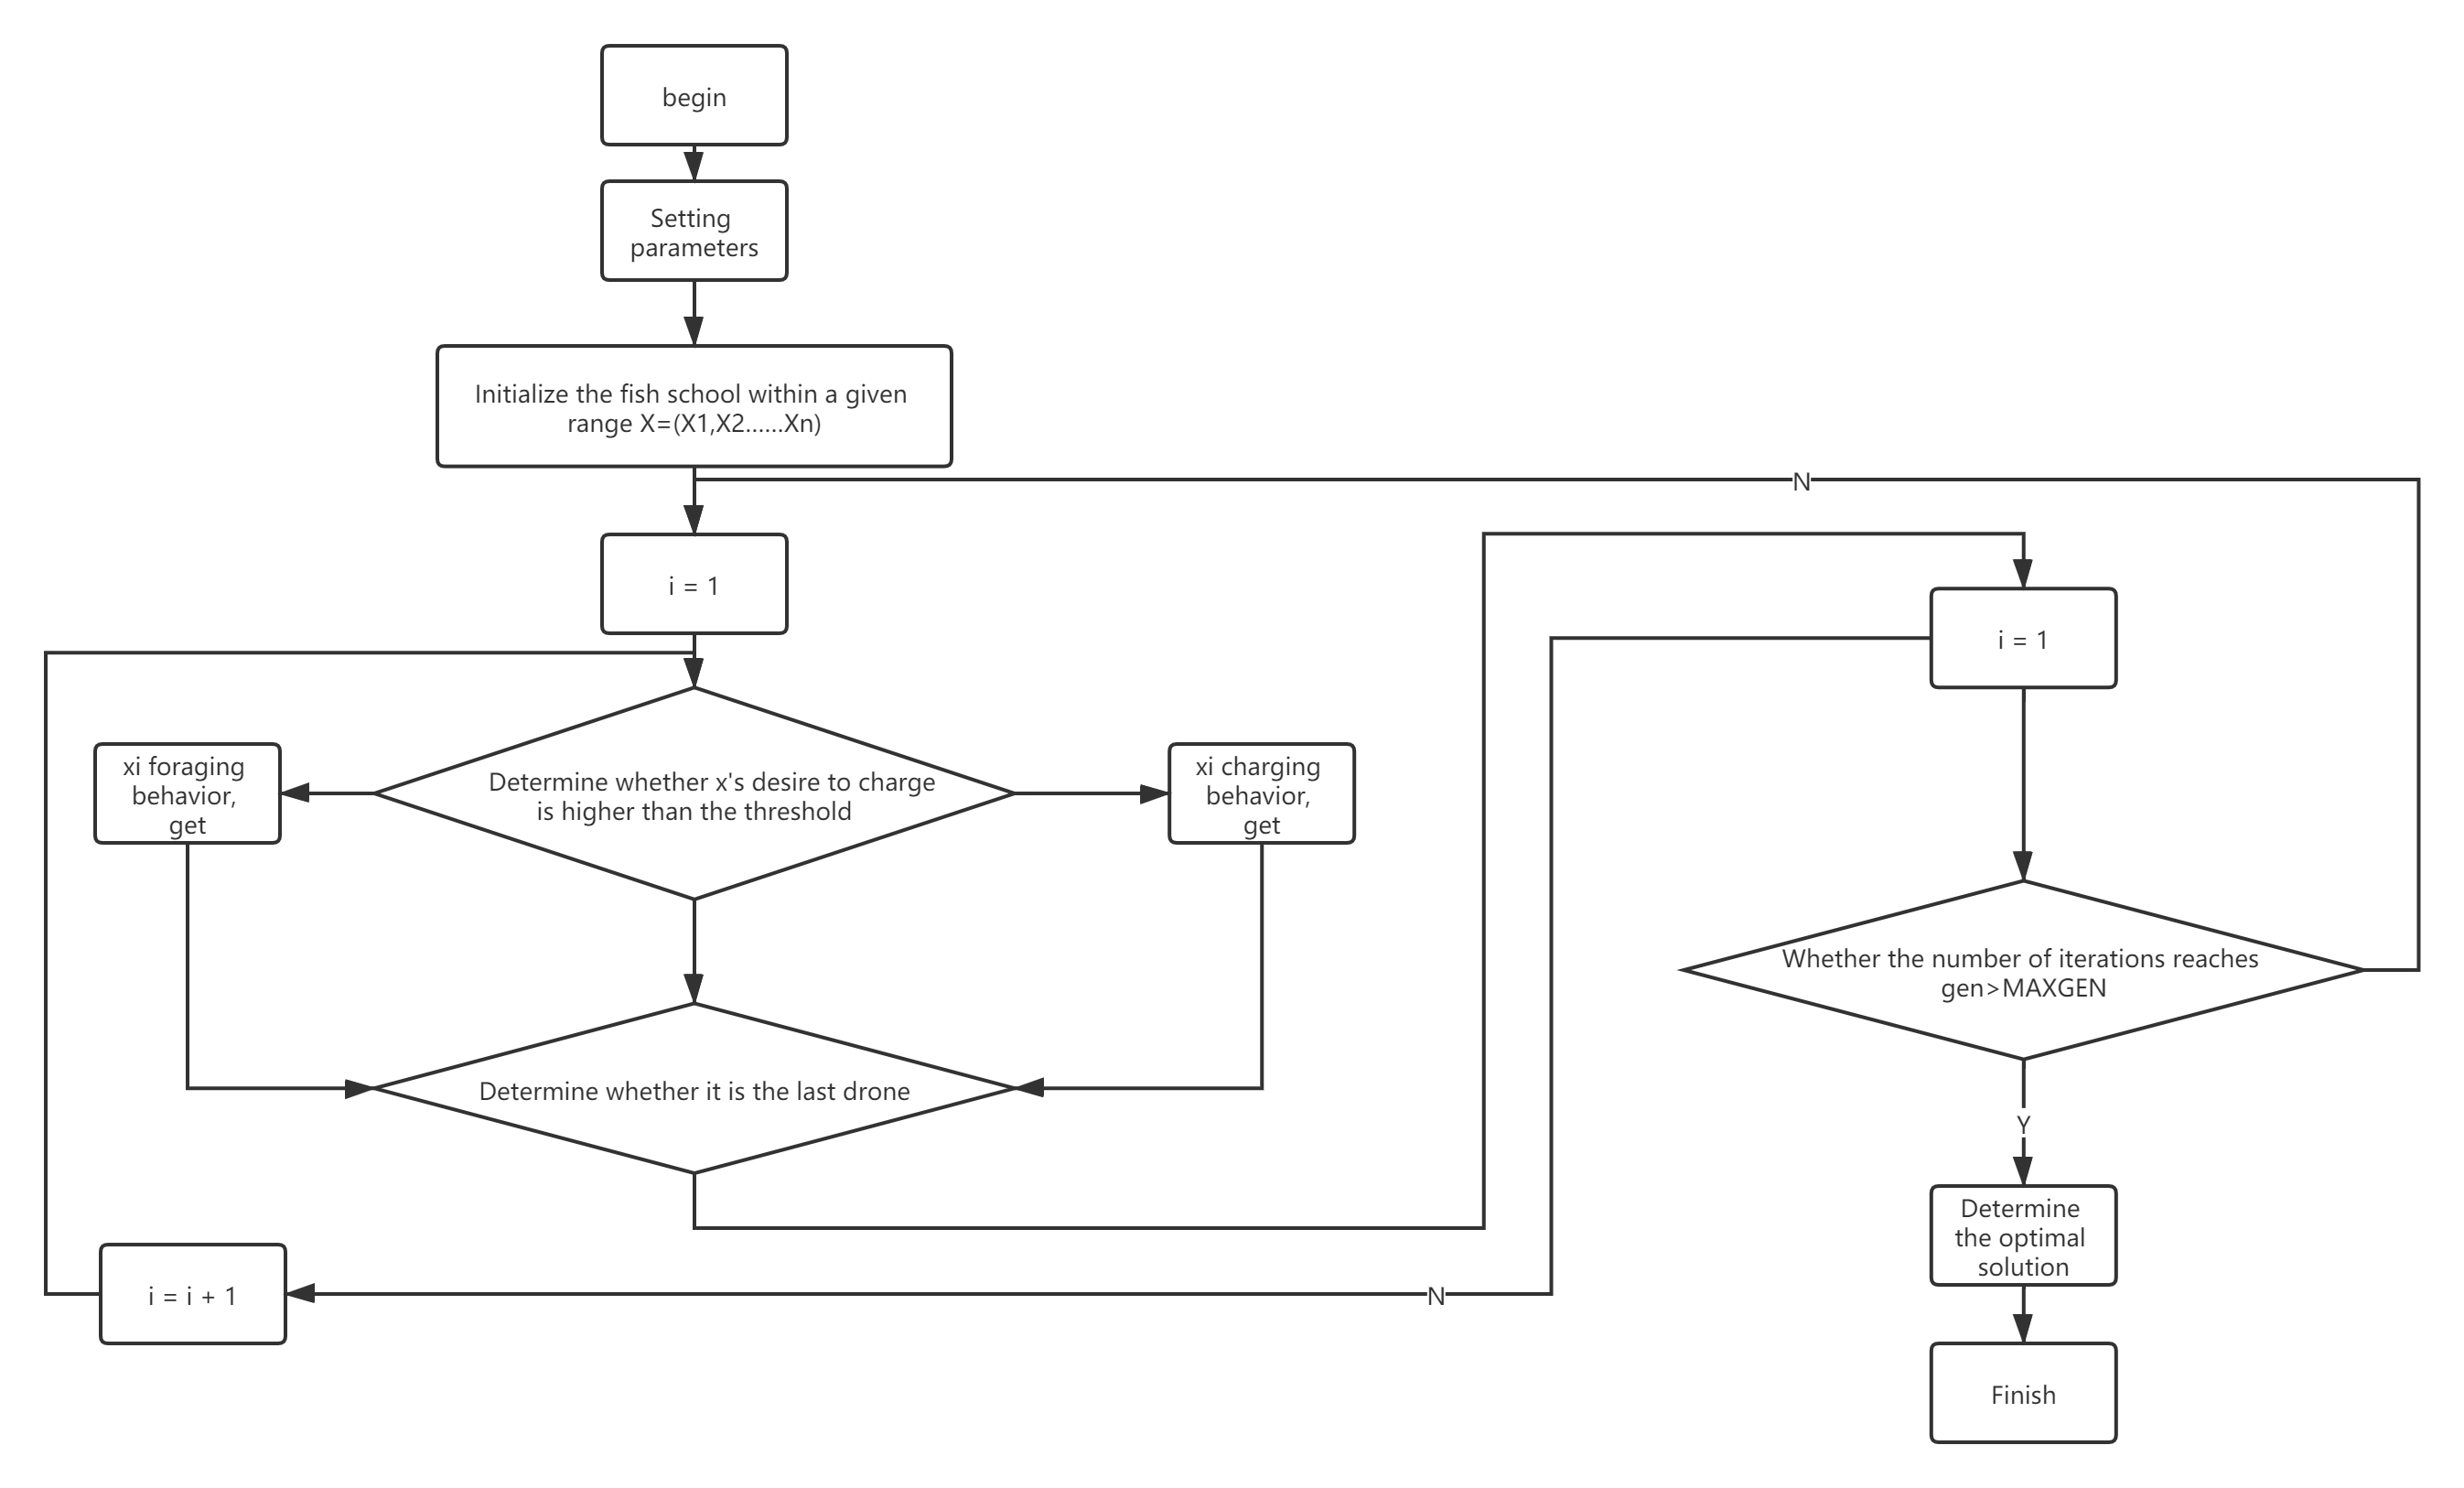
\includegraphics[width=0.9\textwidth]{flow.png}
\caption{Algorithm Flow of Artificial Fish Swarm Planning} % 标题
\label{flow}
\end {figure}


\textbf{\subsection{Model Simulation and Analysis}}

Using the collected data, we perform simulation on our model to simulate flight trajectory of the SSA dones, then analyze the resulting characteristics of this model.

We set the iteration threshold to 500 and test the refreshing rate of each point on the map when the number of SSA drones ranges from 1 to 40.Finally, we get some results about the relationship between the refreshing rate and the number of SSA drones, and produce a thermodynamic diagram as shown in the figure below.

\begin{figure*}[h]
	\centering
	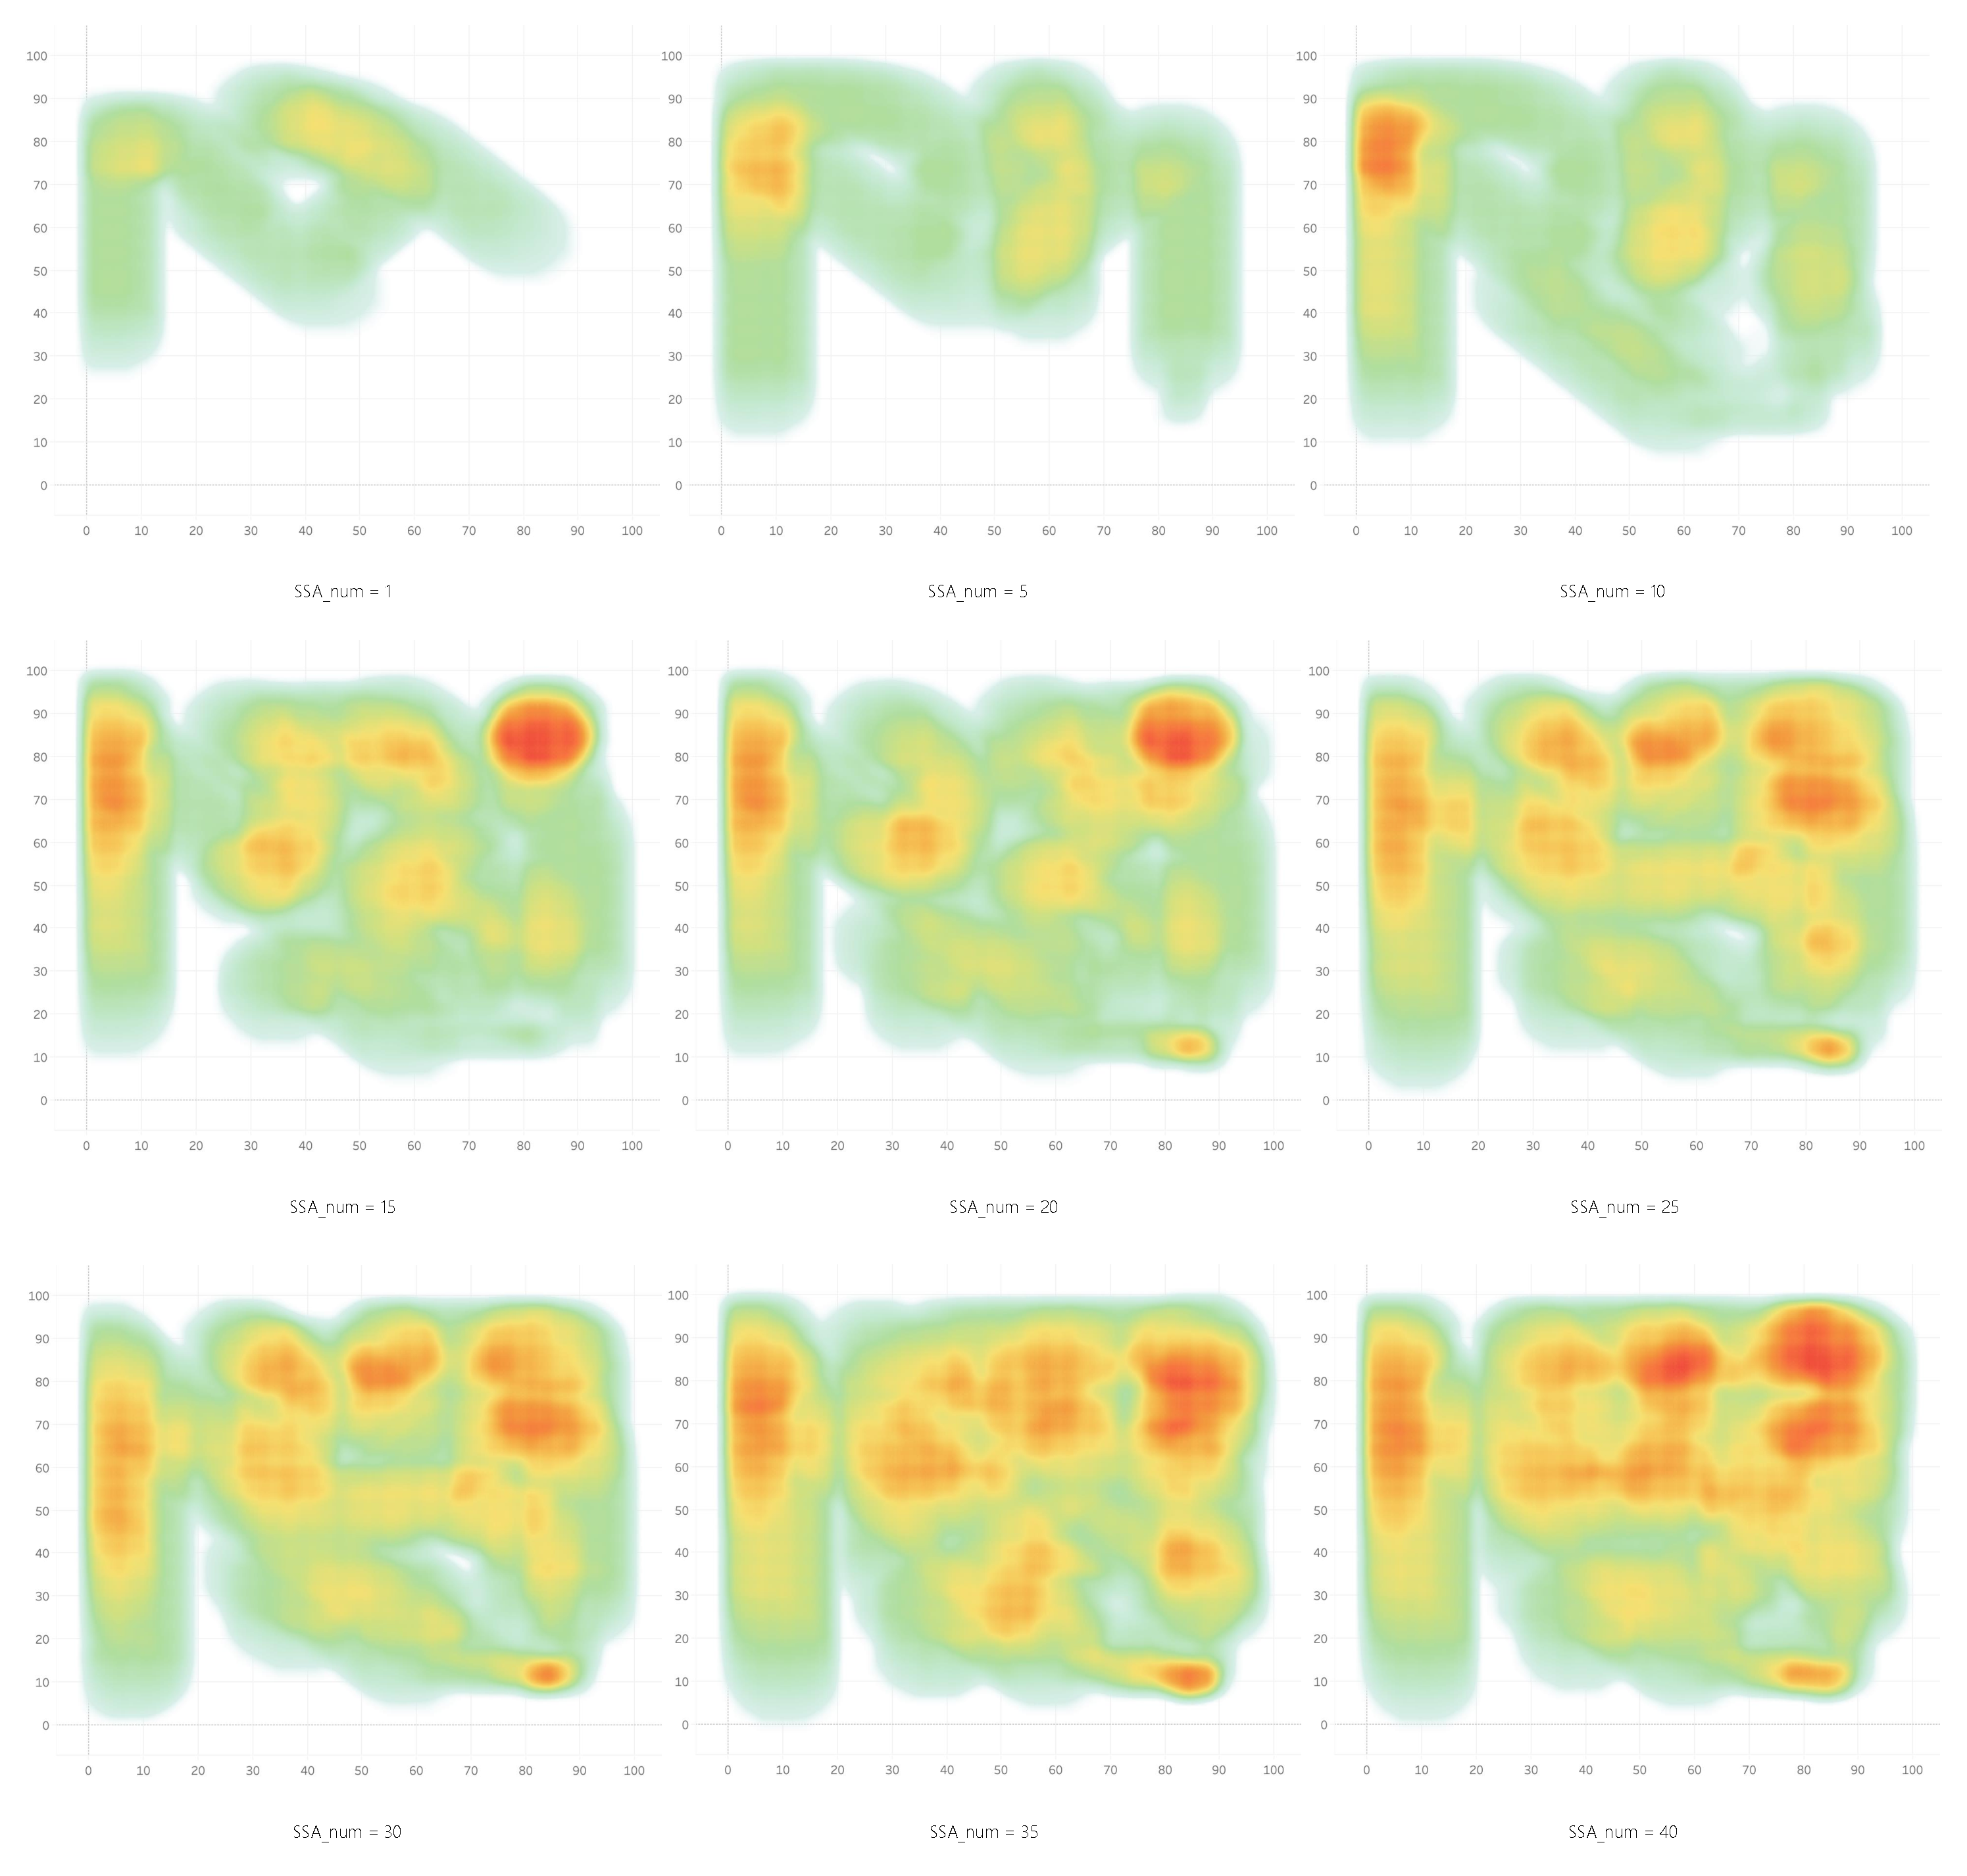
\includegraphics[width=0.9\textwidth]{fig/fig1.pdf}\\
	\vspace{-3mm}
	\caption{Thermodynamic chart of refresh rate of each point on the map}
	\label{fig:fig1}
	\vspace{-4ex}
\end{figure*}

As shown in the Figure \ref{fig:fig1}, the thicker the color, the higher the refresh rate is. With the gradual increase of the number of UAVs, the area covered on the map is gradually becoming larger, indicating that the scope of UAV monitoring is gradually expanding. Besides, according to the distribution of points with high refreshing rate on the map, it can be seen that with the increase of the number of SSA drones, the probability of receiving monitoring (that is, the refresh rate of the location) at the place with high fire incidence is also higher, which meets the logical requirements of on-the-spot observation.

However, by comparing the thermal maps with the number of UAVs ranging from 20 to 40, it can be found that the improvement speed of the map refresh rate is decreasing. Compared with the linear growth of the economic cost, the cost performance of increasing the current monitoring capability of UAVs is lower.

Therefore, only from the perspective of qualitative analysis, 15 SSA UAVs and 4 UAVs equipped with repeaters are needed in the region under the assumption of this paper, so as to realize the global saturated fire monitoring and early warning under the premise of low cost.

Moreover, we output a UAV track image which shows the effect of multi UAVs flying and monitoring together in this model intuitively.
\begin {figure}[h]
\centering % 居中显示
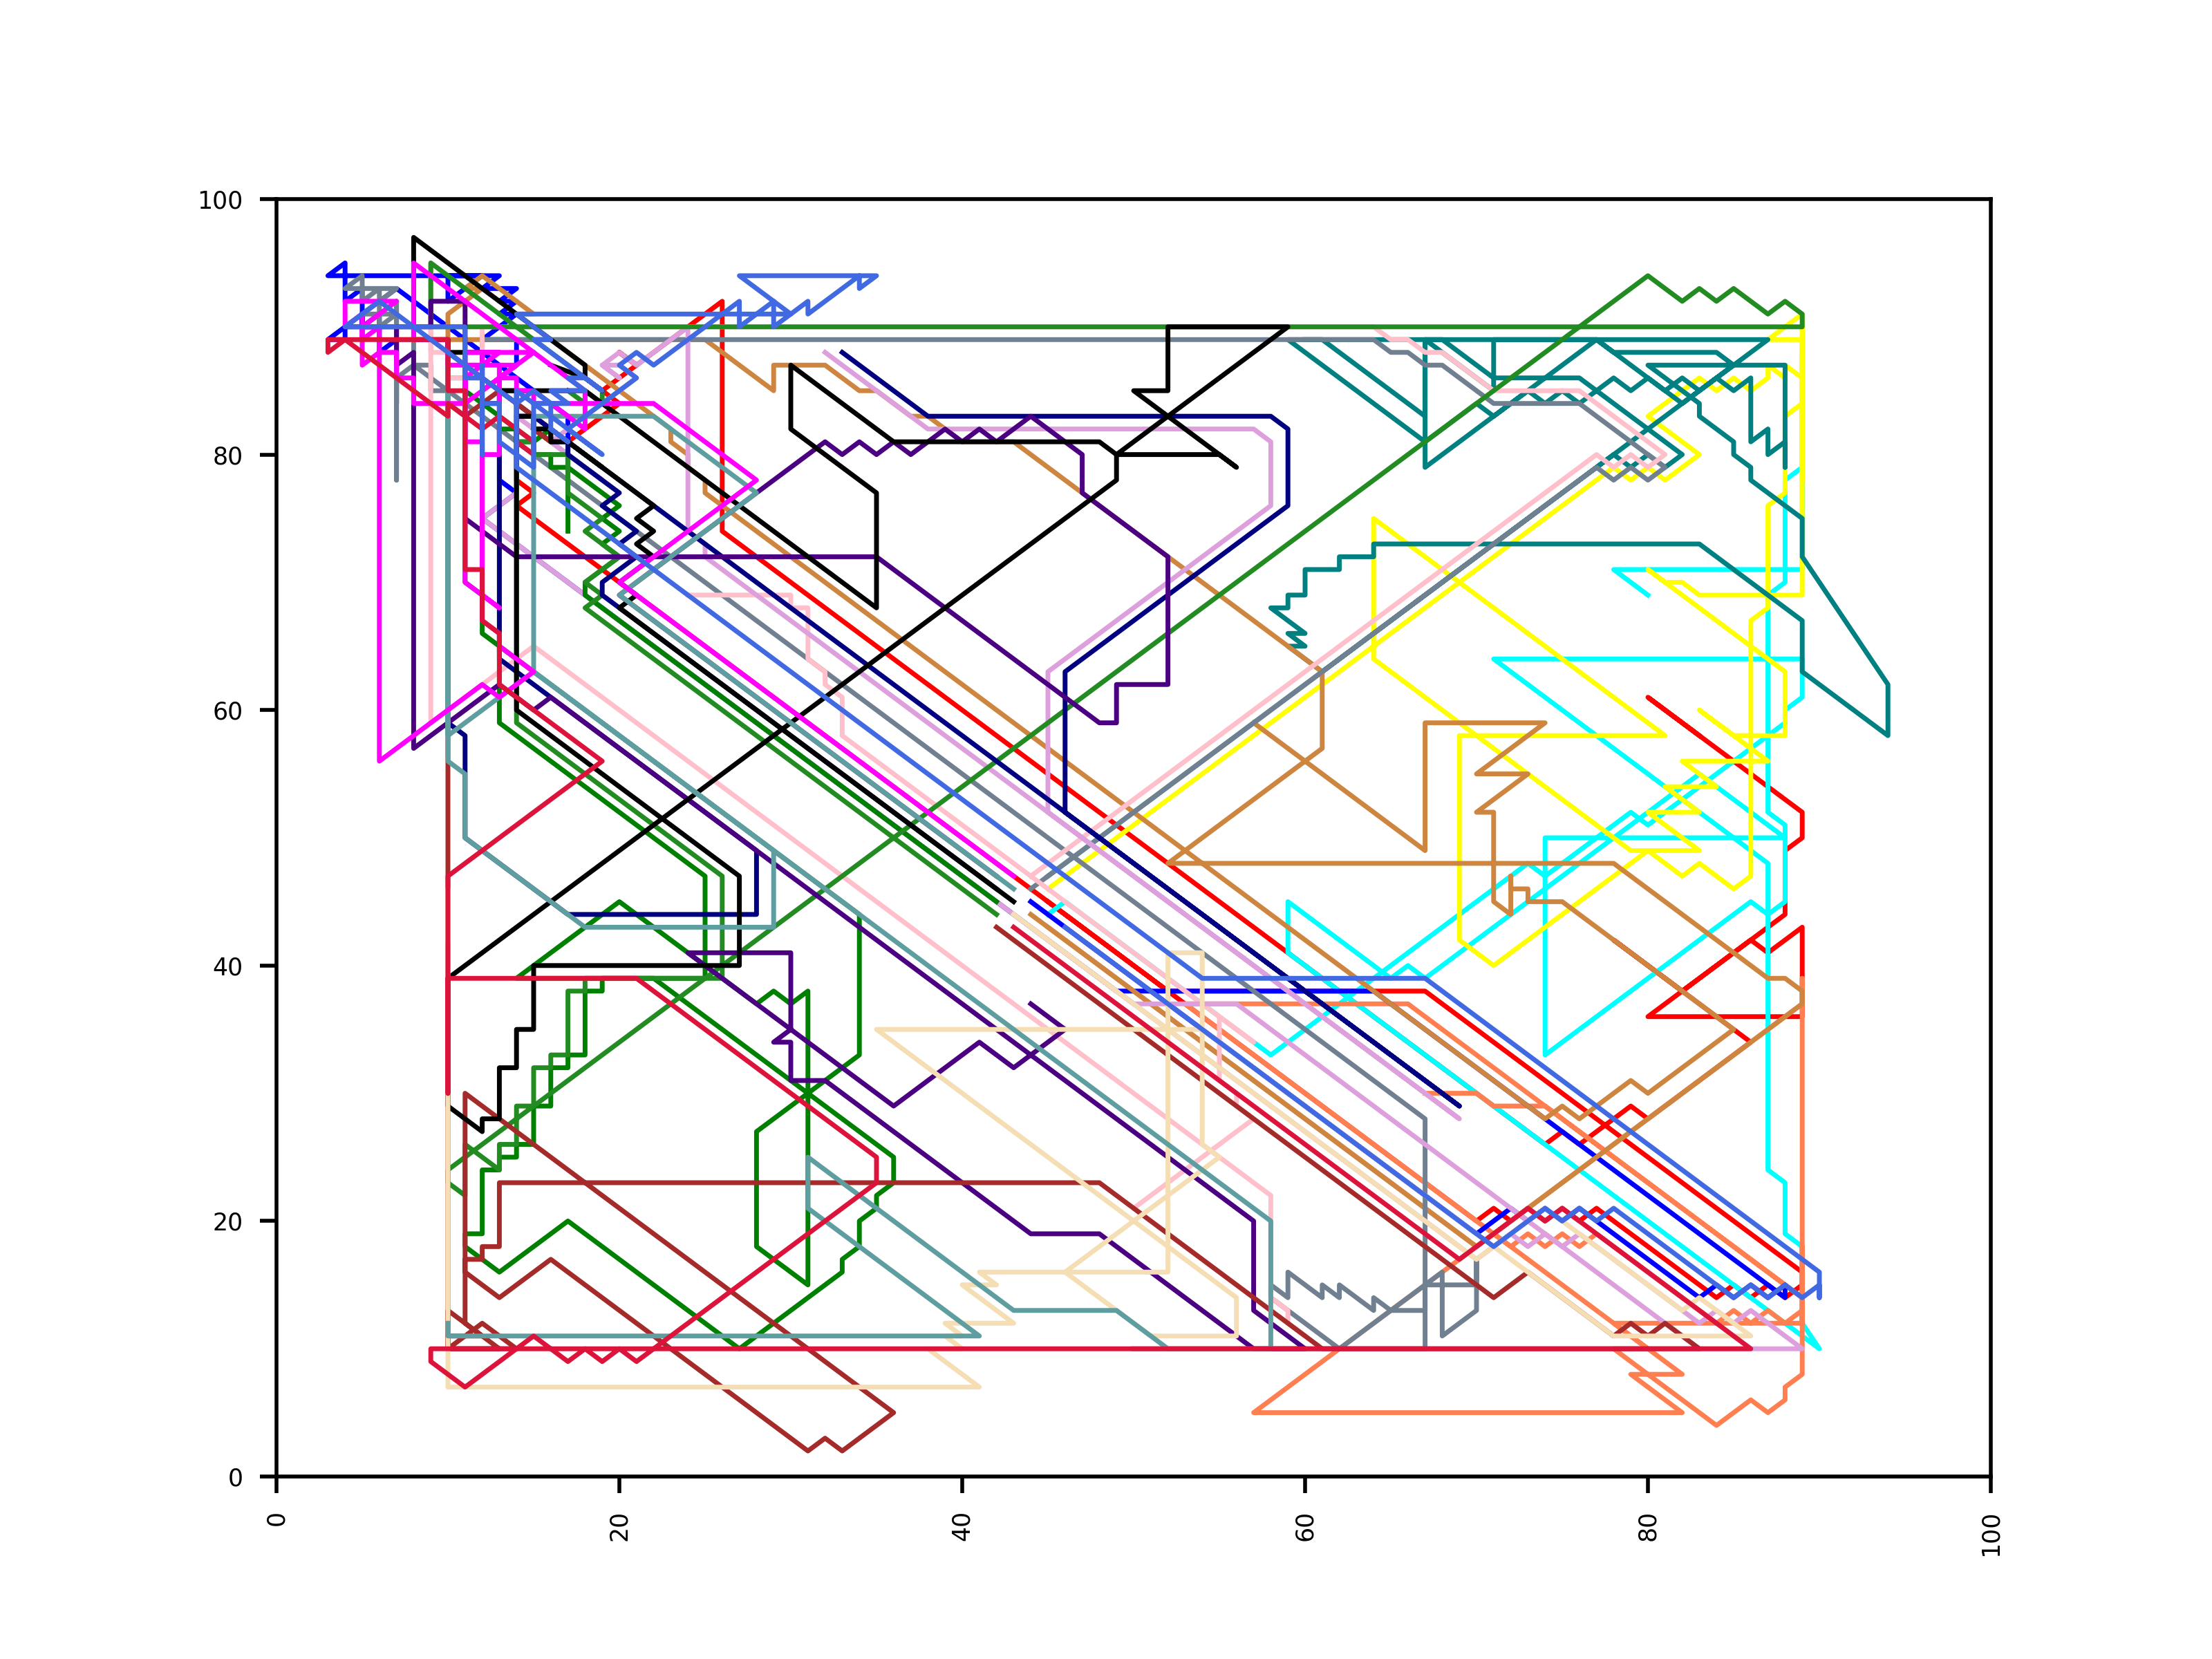
\includegraphics[width=0.9\textwidth]{q1.1.png}
\caption{Dynamic track chart of specified number of SSA drones} % 标题
\label{track}
\end {figure}


\textbf{\section{Forecast of Future Situation(Question 2)}}

\textbf{\subsection{Data Description and Model Adjustment}}

We collecte the data of Australian mountain fire in the past ten years, and use the gray prediction model to predict the probability of fire at each point on the map in the next ten years.
Based on the model we forme in the question 1, we adjust our model to adapt to new problems. By changing the fire frequency dataset, we successfully get the following results in the Figure \ref{fig:q2}.


\begin{figure*}[h]
	\centering
	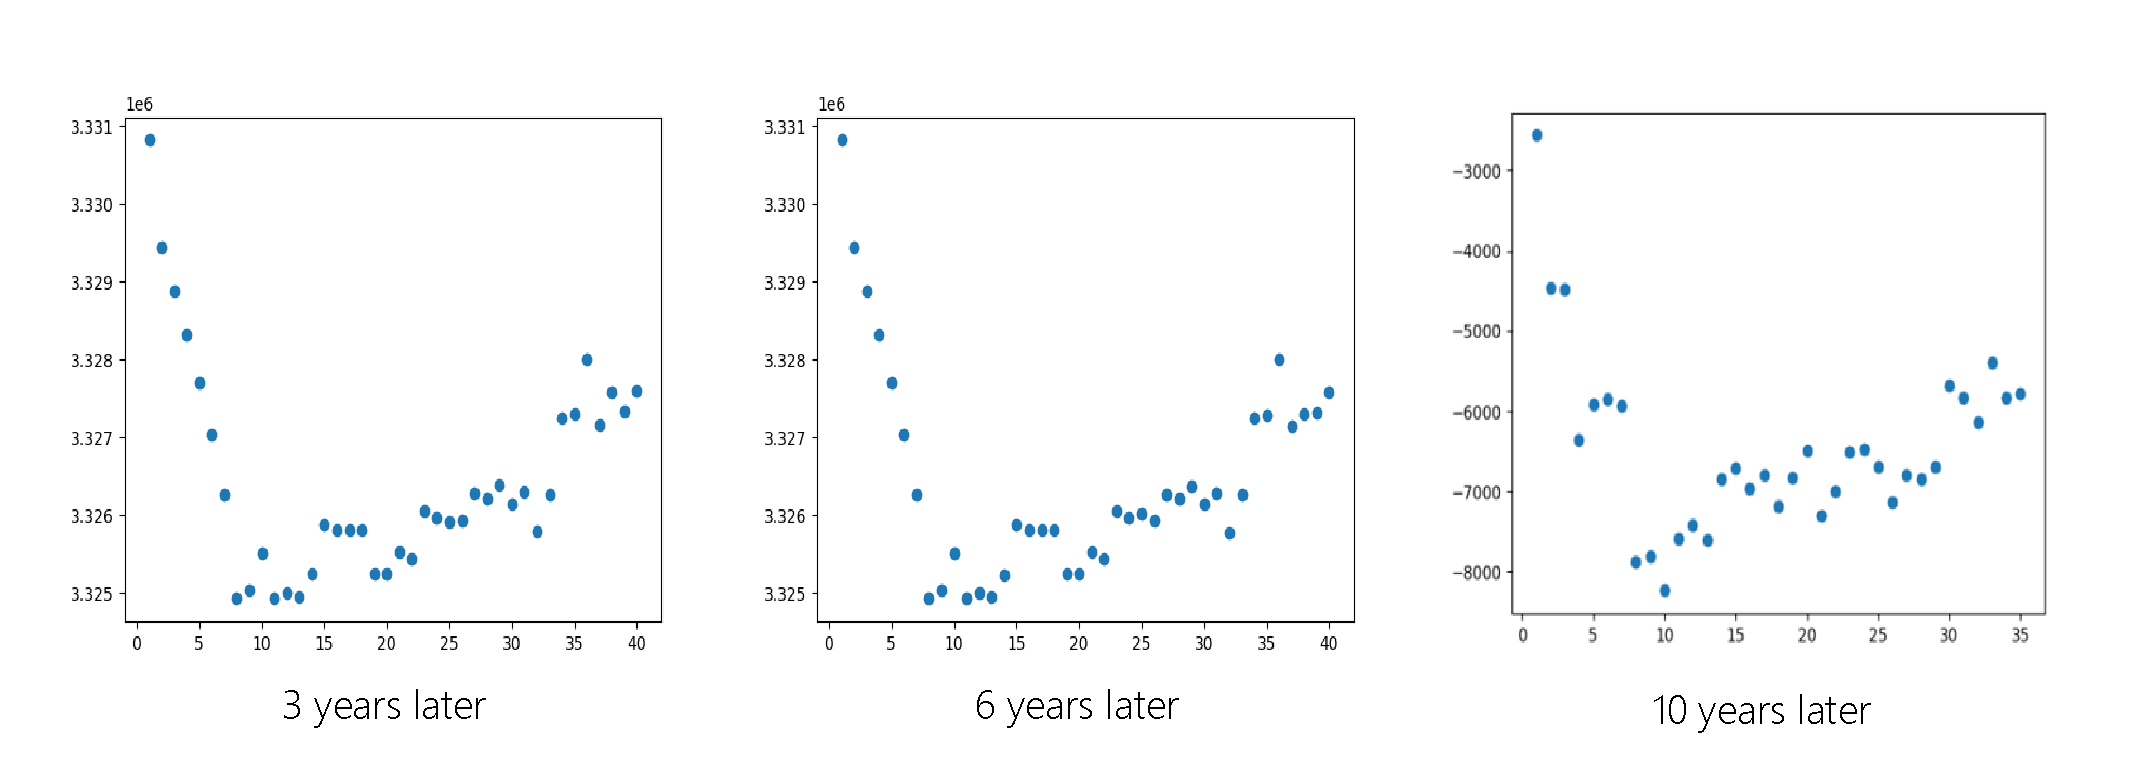
\includegraphics[width=0.9\textwidth]{fig/q2.pdf}\\
	\vspace{-3mm}
	\caption{Model performance in the next decade}
	\label{fig:q2}
	\vspace{-4ex}
\end{figure*}


\textbf{\subsection{Model Simulation and Analysis}}
In the Figure \ref{fig:q2}, we can see that the time nodes in the next three years and the next six years have achieved good planning performance, which is basically consistent with the change trend of the current model, and both maintain a steady growth trend with the increase of the number of UAVs. 

However, with the continuous growth of time, considering the serious fire caused by global warming and other climate factors year by year, the UAV monitoring model still maintaining the current number of configuration has been unable to meet the needs of the corresponding years. In the figure of '10 years later', we can see that the performance indicators have shown abnormal negative values. Therefore, The old parameter setting can not adapt to the changing possibility of extreme fire events in the next decade. 

If you want to restore the performance of this model and continue to use similar schemes to arrange UAVs to monitor the fire, you need to increase the number of UAVs. By increasing the number of UAVs, you can offset the weakening effect of the model caused by the increase of fire probability parameters, so as to make this model come back to life.

Assuming that the cost of UAV system remains unchanged, it is necessary to increase the number of UAVs to adapt to the extreme fire changes in the next decade. Therefore, the increase of equipment cost will have a linear relationship with the increase of the number of UAVs.


\textbf{\section{Repeater Location Optimization(Question 3)}}
\textbf{\subsection{Environment Model Adjusting}}
We consider a cellular system where a UAV provides wireless access to terrestrial mobile devices, serving as an aerial base station. The UAV is placed in an adjustable altitude $h$, aiming to communicate with a ground node either directly or through a terrestrial relay, as illustrated in Figure \ref{repeater}

\begin {figure}[h]
\centering % 居中显示
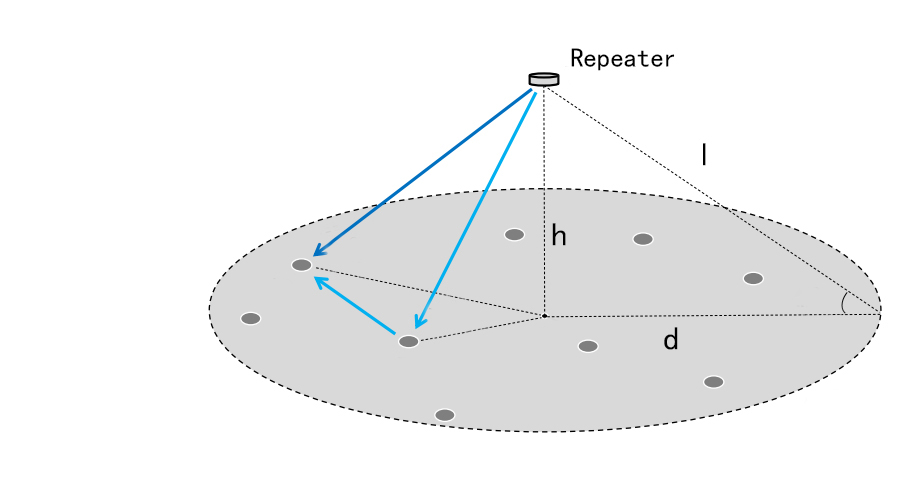
\includegraphics[width=0.9\textwidth]{repeater.jpg}
\caption{A simplified air-to-ground wireless network using a UAV in presence of randomly distributed ground relays over the coverage region, which radius refers to $d$} % 标题
\label{repeater}
\end {figure}

Considering the influence of altitude on repeater signal, we add altitude information $el$ to environment variables based on \textbf{Question 1} environment model.

\textbf{\subsection{Model Optimization}}

On the basis of the original problem route planning model, the constraint conditions are added to the problem three model, so that the location of repeaters can be optimized. 

Determine the repeater signal diameter as $l$ shown in the Figure \ref{repeater}. According to Pythagorean theorem, we gain the following equation:
\begin{equation}
	h^2+d^2=l^2\Rightarrow l=\sqrt{h^2+d^2}
\end{equation}
It is obvious that the value of $l$ is affected by height $h$ while the value of $d$ remains unchanged.So if we want to find the best placement of multiple repeaters, we have to meet the following \textbf{constraints:} 

(1) Assume that repeater $i$ covers a signal range of $d_{i}$, then the corresponding area is $\pi d^2_{i}$. In order to achieve better monitoring effect, multiple repeaters need to cover the largest total area, recorded as:
\begin{equation}
	S_{i}=\sum_{\i=1}^{n}\pi d^2_{i} - \sum_{\i=1}^{n}S_{overlap_{i}}
\end{equation}
$S_{overlap_{i}}$ refers to the overlap of coverage of all the repeaters.

(2) Determine $l_{c_{i}}$ as the distance between the repeater $i$ and the nearest EOC, then the distance condition should satisfy the inequality listed below:
\begin{equation}
	l_{c_{i}} <= d_{i}
\end{equation}

(3) In view of the frequent occurrence area of mountain fire disaster, to ensure the timely monitoring and extinguishing of mountain fires, the relay coverage should be positively correlated with the fire frequency $P_{ff_{i}}$ which means the higher the fire probability, the higher the relay coverage $\eta_{r_{i}}$.

The model of \textbf{Question 3} is optimized by traditional artificial fish swarm algorithm. The artificial fish of this model represents the position information of the repeater, which is the feasible solution we need. After several iterations, the optimized repeater position can be obtained.

\textbf{\subsection{Model Stimulation and Analysis}}
Using the collected terrain data, we perform simulation on our model to simulate hovering positions of UAVs with repeaters, then analyze the resulting characteristics of this model.

We set the iteration threshold to 500 and test the hovering positions corresponding to the point on the map when the number of SSA drones ranges from 1 to 40. We gain a figure showing all the positions of the hovering drones, as illustrated in Figure \ref{q3.1}

For the terrain information mentioned in the stem, the optimal solution can be obtained within the number of iterations, and the optimized repeater position can be obtained after multiple iterations.

\begin {figure}[h]
\centering % 居中显示
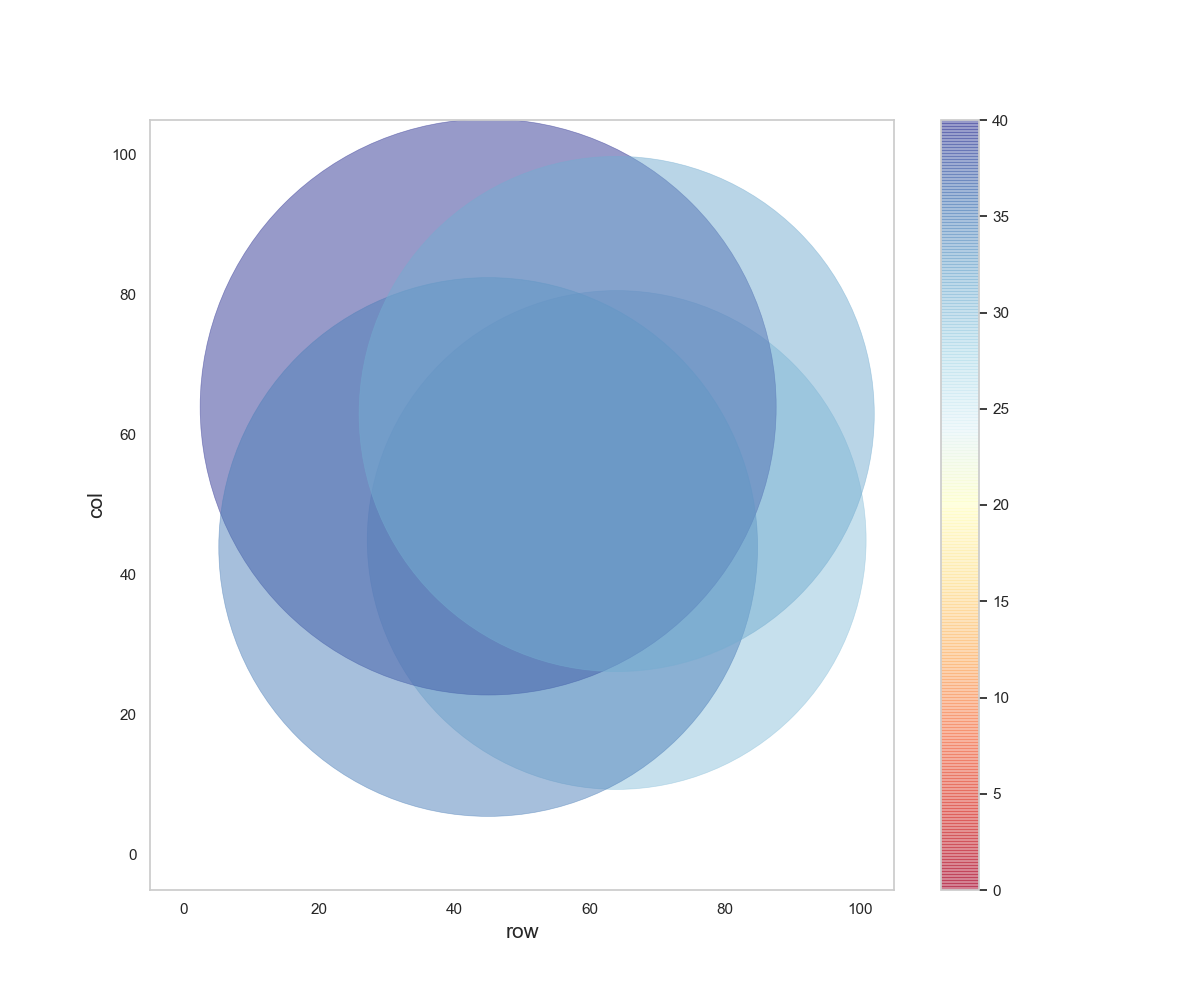
\includegraphics[width=0.9\textwidth]{q3.1.png}
\caption{Hovering positions of UAVs with repeaters} % 标题
\label{q3.1}
\end {figure}


\textbf{\section{Strengths, Weaknesses and Future Discussion}}
Based on the modeling process, we make some comments on our model as listed below.
\textbf{\subsection{Strengths}}
\begin{itemize}
	\item Our model is formulated on a certain theoretical basis. After consulting a large number of literature, we have carefully selected the parameters of the model. In this way, we can make our model as close to reality as possible.
	Considering the actual conditions, we selected an appropriate area on the map based on the temperature, fire frequency and the distribution of forests and cities as the terrain reference area for our modeling. The experimental results are good and have high credibility.
	\item Our model is flexible enough to test more situations. We only need to change a few parameters to do deeper research. For example, the model can judge the combination of drones formations by modifying different terrains; and what will be different if we adjusted the drone field of view.
	\item The model can also be tested according to the model of the drone. If a new drone is introduced, it can be recalculated to meet the needs of the department by modifying the corresponding parameters.
\end{itemize}

\textbf{\subsection{Weaknesses}}
\begin{itemize}
	\item Limited to the limitaion of equipment performance, we did not perform more calculations to fit the model, and the quality of the model may not meet our higher expectations.
	\item Ignore the impact of drone flight speed, so the applicability of drones in larger environments needs to be further improved.
	\item In fact, in some cases, some assumptions may be not hold. There still be some controversy about our model.
\end{itemize}

\textbf{\subsection{Future Discussion}}

We tried to use simulation methods to simulate the flight status of the drone group. However, due to time constraints, we have made many assumptions about the actual situation. For example, regardless of the effect of flame on the drone, the environment around the drone is regarded as unchanged, and so on. Next, we can try to release some assumptions to make the drone combination more flexible. We can explore more possibilities by changing some parameters of the program and adding more rules.

\textbf{\section{Sensitivity Analysis}}

Through the above analysis, we have got the best UAV formation situation. At the same time, we simplified many parameters in the model. In order to ensure the robustness of the algorithm, we mainly tested the model from the following aspects. (Due to time constraints, only the observation field is analyzed this time)
First of all, the probability of fire in different areas will have an impact on the flight status of the drone. The greater the probability of a fire, the easier the drone will travel.
Second, the UAV's field of view has a certain degree of influence on efficiency.
The model we designed allows us to change these parameters. Next, we will analyze in detail the influence of the field of view on the model.
Under ideal experimental conditions, the drone can fly freely without gathering, and set the drone to move at the highest speed.
Set the field of view to 10 and 20 respectively, and check the result of the image change, the result is shown in the figure below:

\begin{figure*}[htb]
	\centering
	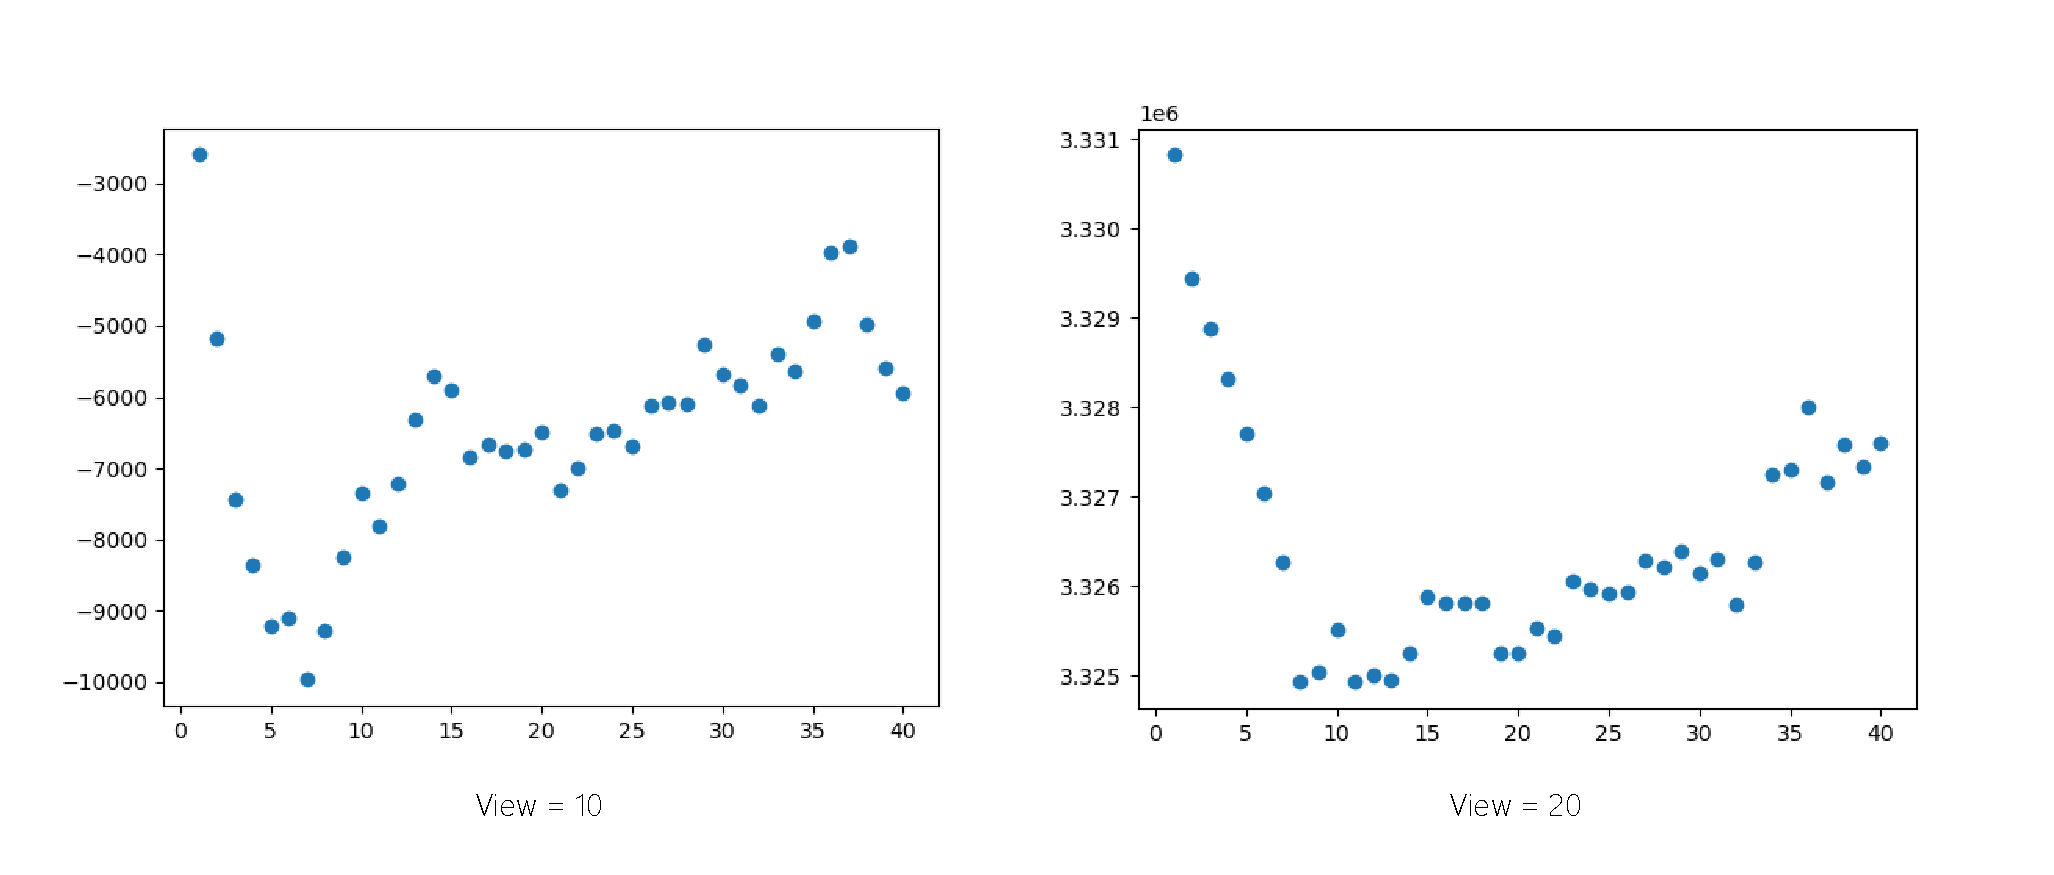
\includegraphics[width=0.9\textwidth]{fig/sensitivity.pdf}\\
	\vspace{-3mm}
	\caption{Model performance in the next decade}
	\label{fig:sensitivity}
	\vspace{-2ex}
\end{figure*}

It can be seen from the above data that these parameters have a certain degree of influence on stability.
The analysis result of the field of view indicates that a larger field of view can be beneficial to the stability of the UAV. Choosing the largest possible field of view for observation is of great benefit to UAV monitoring.
In addition, the analysis results of fire probabilities in different areas show that different probabilities have a greater impact on the flight situation of UAVs.


Both the continuous and periodical inflows lead to increase in the number of opioids in the state. The result shows that the continuous inflow of opioids has the greatest impact. Although the indirect inflows are incidents, they should also raise the government's concern. In conclusion, the government should not only impose strict regulations on opioids inside the state, but also pay attention to the inflow of opioids from outside the state, and monitors the logistics constantly.


\textbf{\section{Conclusion}}
In our experiments, we designed a drone trajectory model based on artificial fish swarm algorithm. The model simulates the use of drones. First, we built a model while balancing safety and economy, and simulated the best formation of drones. It is found that under certain conditions, 4 radio repeater drones and 15 SSA drones are the optimal combination. Then use the grey prediction model to predict the fire situation in the next ten years, combined with the fire situation prediction, the existing combination is not enough to meet the demand ten years later, the number of drones needs to be increased, so the budget has increased. Then we discuss the influence of terrain on the layout of radio repeater drones in combination with terrain. After sensitivity analysis, the results have good robustness and the results are credible. 
Although our model has good scalability and flexibility, it still has certain flaws. There are too many assumptions, so there is still a certain gap between the model and the actual situation. 
However, we discussed some practical ways to improve the reliability of the results. For example, how to achieve the charging state, how to choose a suitable initial location and so on. In the future, we still have the opportunity to continue to optimize our model.

\newpage
\textbf{ \section*{\centerline{Annotated Budget Request}}\addcontentsline{toc}{section}{Annotated Budget Request}}
\fancyhf{}
\fancyhead[R]{ }
\fancyhead[L]{ }

\begin{flushright}
	Team \# 2106317 \\
	MCM/ICM Contest \\
	Problem B \\
	February 8,2021 \\
\end{flushright}

\begin{flushleft}
	From CFA \\
	To the Victoria State Government
\end{flushleft}
\pagestyle{empty}%
\large%
\begin{center}
	\begin{tabular}{l l}%
		\hline%
		\hline%
		\textit{Item*Number}&\textit{Price}\\%
		\hline%
		WileE–15.2X Hybrid Drone * 209& \textbf{\$ 10000}\\%
		\hline%
		Total&\textbf{\$ 2.09 million}\\%
		\hline%
		\hline%
	\end{tabular}%内容...
\end{center}

\textbf{\subsection*{\centerline{Description}}}

\textbf{\subsection*{1、Backgroud}}
From 2019 to 2020, devastating wildfires occurred in all states of Australia, with the worst impact in New South Wales and eastern Victoria. Tomonitor the fire, firefighters have used drones for surveillance and situational awareness (SSA). Drones are divided into SSA drones and Radio Repeater drones. It is necessary to design the number of drones and the combination of drone formations.
\textbf{\subsection*{2、Requirements}}
In order to face frequent  devastating wildfires, we will set up a new department "Rapid Bushfire Response" to purchase new equipment to respond future needs. We use the artificial fish swarm algorithm to estimate and find that the best combination of a group of drones is four Radio Repeater drones and fifteen SSA drones to ensure the monitoring of the fire range and the safety of personnel. We have also considered the actual situation in Victoria, balanced economy and safety, and believed that eleven groups of drones should be purchased to deal with future extreme wildfires. 
\textbf{\subsection*{3、Budget}}
a total of 273 drones will be purchased. The cost of a drone is about \$10,000, so all of them will cost \$2.09 million.
\textbf{\subsection*{4、Usage}}
These drones will be used to detect bush fires. We will deploy these drones in cities near forests and surrounding fire-prone cities to prevent fires and quickly go to the fire scene when a fire occurs. Observe the situation. SSA drones can not only be used to monitor the situation of the fire scene, but also can monitor the wearable devices of frontline personnel to further ensure the safety of forward teams. The radio repeater drone expands the radio transmission range and can help front-line personnel get information about the fire better.
\textbf{\subsection*{5、Conclusion}}
We believe that the purchase of these drones is enough to complete the monitoring of fires, while balancing economy and safety. It should be noted that these drones are vital to the future development trend of fires. We hope to purchase drones through budgeting as soon as possible.


% 因为不输出此部分到目录 \addcontentsline{}{}{}是添加此标题到目录 
\newpage
\textbf{\section*{References}}\addcontentsline{toc}{section}{References}
\begin{thebibliography}{99}  
	\bibitem{ref1}R. Li, S. Pan, H. Fang, Y. Xiong and F. Wang, "Fault Prediction Technology of Civil Aircraft Based on Qar Data," 2017 International Conference on Sensing, Diagnostics, Prognostics, and Control (SDPC), Shanghai, 2017, pp. 468-472, doi: 10.1109/SDPC.2017.94.
	\bibitem{ref2}Z. Xiao, P. Xia and X. Xia, "Enabling UAV cellular with millimeter-wave communication: potentials and approaches," in IEEE Communications Magazine, vol. 54, no. 5, pp. 66-73, May 2016, doi: 10.1109/MCOM.2016.7470937.
	\bibitem{ref3} C. Zhang and W. Zhang, "Spectrum Sharing for Drone Networks," in IEEE Journal on Selected Areas in Communications, vol. 35, no. 1, pp. 136-144, Jan. 2017, doi: 10.1109/JSAC.2016.2633040.
	\bibitem{ref4}L. Gupta, R. Jain and G. Vaszkun, "Survey of Important Issues in UAV Communication Networks," in IEEE Communications Surveys \& Tutorials, vol. 18, no. 2, pp. 1123-1152, Secondquarter 2016, doi: 10.1109/COMST.2015.2495297.
	\bibitem{ref5}Li Shoujun.Grey Forecasting Model Based on Fuzzy Sets and It Application[D].Jiangsu:China University of Mining and Technology,2018.
\end{thebibliography}

%\fancyhf{}
%\fancyhead[R]{ }
%\fancyhead[L]{ }
%\bibliography{books}
%\Large
%\bibliographystyle{IEEEtran}

\newpage
\textbf{\section*{Appendices}\addcontentsline{toc}{section}{Appendices for Code and Data}} 
\fontsize{13pt}{12.5pt}\selectfont
Here is Code we used in our model, which python is the main development language.
\vspace{7pt}
\textbf{\subsection*{Appendices: The Program for Calculating Performance}}
\noindent{\rule{\textwidth}{0.2mm}}
\vspace{-18pt} 
\fontsize{13pt}{12.5pt}\selectfont
{
	\lstinputlisting[language=python]{matrix.py}
}
\vspace{-15pt}
\noindent{\rule{\textwidth}{0.2mm}}
\vspace{-15pt}
\noindent{\rule{\textwidth}{0.2mm}}

\end{document}